
% Stereographic and cylindrical map projections
% Author: Tomasz M. Trzeciak
% Source: LaTeX-Community.org 
%         <http://www.latex-community.org/viewtopic.php?f=4&t=2111>


\documentclass{standalone}
\usepackage{tikz}
\usetikzlibrary{intersections,calc,fadings,decorations.pathreplacing}
\usepackage{verbatim}
\usepackage{xparse}

:Title: Stereographic and cylindrical map projections
:Tags: 3D
:Slug: map-projections
:Grid: 2x2

Examples inspired by the thread at comp.text.tex about `how to convert some hand
drawn pictures into programmatic 3D sketches`__.

.. __: http://groups.google.com/group/comp.text.tex/browse_thread/thread/a03baf5d6fa64865/f7e7b903f1d87a6a

The sketches present stereographic and cylindrical map projections and they
pose some interesting challenges for doing them with a 2D drawing package PGF/TikZ.

The main idea is to draw in selected 3D planes and then project onto the canvas
coordinate system with an appriopriate transformation. Some highlights:

- usage of pgf math engine for calculation of projection transformations and
  transitions points from visible (solid lines) to invisible (dashed lines) on
  meridians and latitude circles
- definition of 3D plane transformation with expanded styles so that they are robust
  against redefinition of macros used in their construction
- usage of named coordinates (nodes) for definition of characteristic points in
  local coordinate systems so that they are accessible outside of their plane of
  definition
- calculation of intersections points with TikZ intersection coordinate system
- usage of 'to' path operation instead of 'arc' for marking angles to allow for
  easy positioning of text labels on the curve
- 3D lighting effects with shading

:Author: Tomasz M. Trzeciak
:Source: LaTeX-Community.org_

.. _LaTeX-Community.org: http://www.latex-community.org/viewtopic.php?f=4&t=2111



%% helper macros

\newcommand\pgfmathsinandcos[3]{%
  \pgfmathsetmacro#1{sin(#3)}%
  \pgfmathsetmacro#2{cos(#3)}%
}
\newcommand\LongitudePlane[3][current plane]{%
  \pgfmathsinandcos\sinEl\cosEl{#2} % elevation
  \pgfmathsinandcos\sint\cost{#3} % azimuth
  \tikzset{#1/.style={cm={\cost,\sint*\sinEl,0,\cosEl,(0,0)}}}
}
\newcommand\LatitudePlane[3][current plane]{%
  \pgfmathsinandcos\sinEl\cosEl{#2} % elevation
  \pgfmathsinandcos\sint\cost{#3} % latitude
  \pgfmathsetmacro\yshift{\cosEl*\sint}
  \tikzset{#1/.style={cm={\cost,0,0,\cost*\sinEl,(0,\yshift)}}} %
}
\newcommand\DrawLongitudeCircleName[3][1]{
  \LongitudePlane{\angEl}{#2}
  \tikzset{current plane/.prefix style={scale=#1}}
   % angle of "visibility"
  \pgfmathsetmacro\angVis{atan(sin(#2)*cos(\angEl)/sin(\angEl))} %
  \draw[name path=#3,current plane] (\angVis:1) arc (\angVis:\angVis+180:1);
  \draw[name path=dashed#3,current plane,dashed] (\angVis-180:1) arc (\angVis-180:\angVis:1);
}
\newcommand\DrawLatitudeCircleName[3][2]{
  \LatitudePlane{\angEl}{#2}
  \tikzset{current plane/.prefix style={scale=#1}}
  \pgfmathsetmacro\sinVis{sin(#2)/cos(#2)*sin(\angEl)/cos(\angEl)}
  % angle of "visibility"
  \pgfmathsetmacro\angVis{asin(min(1,max(\sinVis,-1)))}
  \draw[name path=#3,current plane] (\angVis:1) arc (\angVis:-\angVis-180:1);
  \draw[name path=dashed#3,current plane,dashed] (180-\angVis:1) arc (180-\angVis:\angVis:1);
}

%% document-wide tikz options and styles

\tikzset{%
  >=latex, % option for nice arrows
  inner sep=0pt,%
  outer sep=2pt,%
  mark coordinate/.style={inner sep=0pt,outer sep=0pt,minimum size=3pt,
    fill=black,circle}%
}

\begin{document}

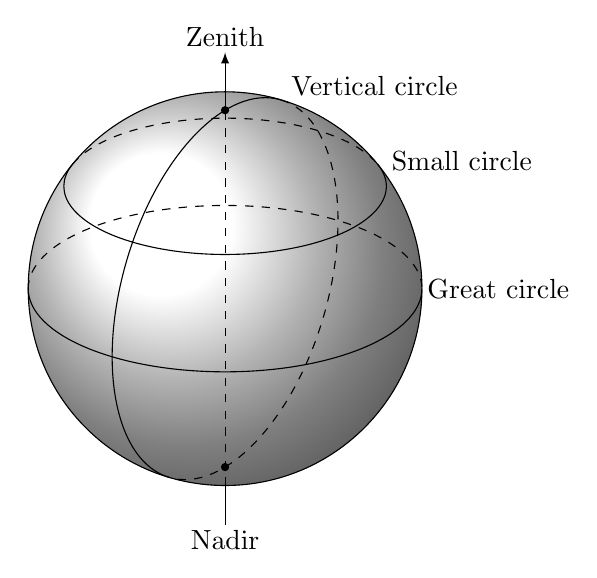
\begin{tikzpicture} % "THE GLOBE" showcase

\def\R{2.5} % sphere radius
\def\angEl{25} % elevation angle
\filldraw[ball color=white] (0,0) circle (\R);
\DrawLatitudeCircleName[\R]{0}{lat1}
\DrawLatitudeCircleName[\R]{35}{lat2}
\DrawLongitudeCircleName[\R]{-125}{lon}
%\DrawLongitudeCircle[\R]{-50}{lon2}
%\foreach \t in {-80,-60,...,80} { \DrawLatitudeCircle[\R]{\t} }
%\foreach \t in {-5,-35,...,-175} { \DrawLongitudeCircle[\R]{\t} }

% Find the intersection points and mark them with dots
%\path[name intersections={of = lat and lon1,by={a}}];
%\path[name intersections={of = lat and lon2,by={b}}];
%\node[mark coordinate, label={above right: $A'$}] at (a) {};
%\node[mark coordinate, label={above left: $B'$}] at (b) {};

\pgfmathsetmacro\H{\R*cos(\angEl)} % distance to north pole
\coordinate (O) at (0,0);
\coordinate[mark coordinate] (Z) at (0,\H);
\coordinate[mark coordinate] (N) at (0,-\H);
\coordinate (greatcircle) at (0:\R);
\coordinate (smallcircle) at (35:\R);
\coordinate (verticalcircle) at (72:\R);
%\coordinate[mark coordinate] (a) at (229:0.525*\R);
%\coordinate[mark coordinate] (b) at (333:0.72*\R);

%\node[above=8pt] at (Z) {Zenith};
%\node[below=8pt] at (N) {Nadir};
\draw[dashed] (0,-\R) -- (0,\H);
\draw[->] (0,\H) -- (0,1.2*\R) node[above] {{Zenith}};
%\draw[dashed] (0,-\H) -- (0,-\R);
\draw (0,-\R) -- (0,-1.2*\R) node[below] {{Nadir}};
%\node[below right] at (O) {$O$};
\node[right] at (greatcircle) {{Great circle}};
\node[above right] at (smallcircle) {{Small circle}};
\node[above right] at (verticalcircle) {{Vertical circle}};
%\draw (a) node[above right] {$A$};
%\draw (b) node[above left] {$B$};
%\draw (Z) node[left 3pt] {$C$};
%\node[label={[label distance=5pt]-60:$C$}] {};
%\node[label={2:$C'$}] at (Z) {};
%\node[label={below : $C$}] at (Z) {};
%\node[label={[xshift=-0.3cm,yshift=-0.40cm]$C'$}] at (Z) {};
%\draw[blue] (a) to (b);



\end{tikzpicture}

\begin{comment}
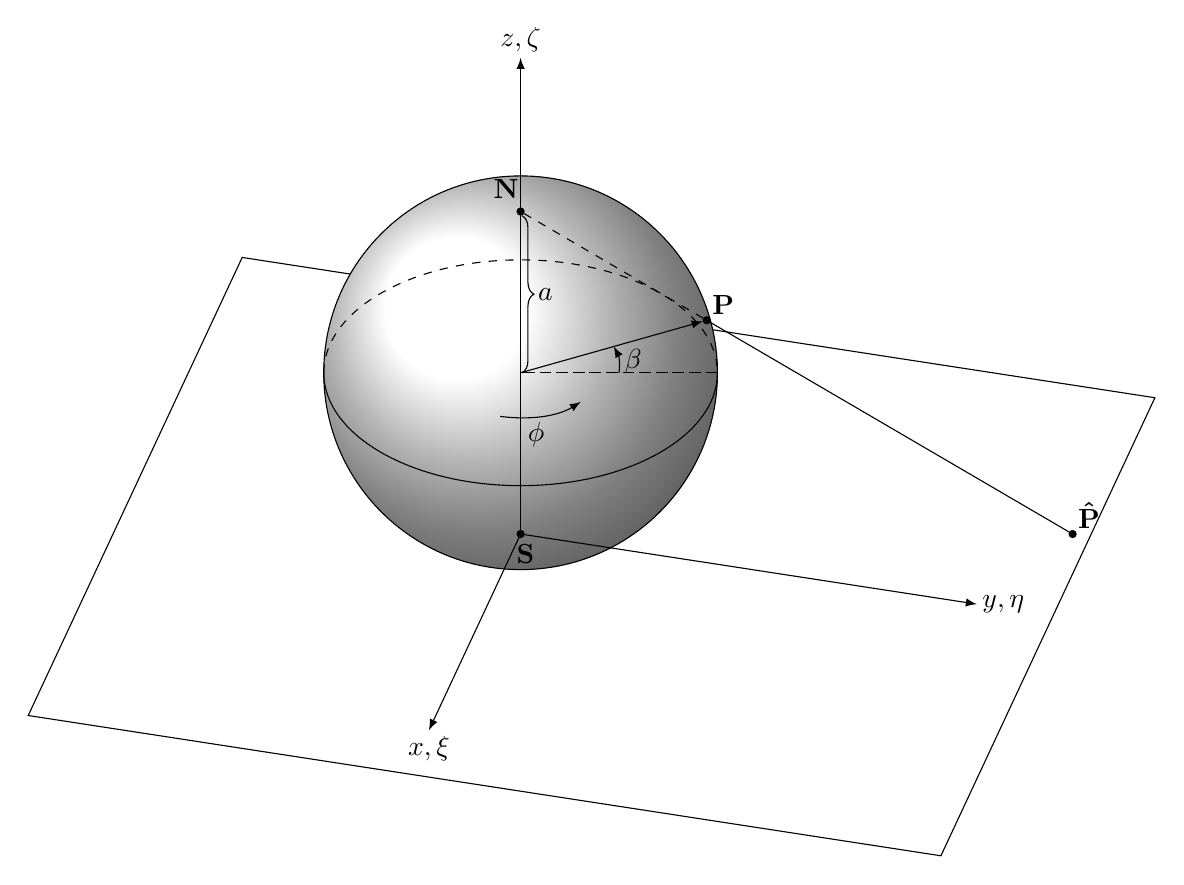
\begin{tikzpicture} % CENT

%% some definitions

\def\R{2.5} % sphere radius
\def\angEl{35} % elevation angle
\def\angAz{-105} % azimuth angle
\def\angPhi{-40} % longitude of point P
\def\angBeta{19} % latitude of point P

%% working planes

\pgfmathsetmacro\H{\R*cos(\angEl)} % distance to north pole
\tikzset{xyplane/.estyle={cm={cos(\angAz),sin(\angAz)*sin(\angEl),-sin(\angAz),
                              cos(\angAz)*sin(\angEl),(0,-\H)}}}
\LongitudePlane[xzplane]{\angEl}{\angAz}
\LongitudePlane[pzplane]{\angEl}{\angPhi}
\LatitudePlane[equator]{\angEl}{0}

%% draw xyplane and sphere

\draw[xyplane] (-2*\R,-2*\R) rectangle (2.2*\R,2.8*\R);
\fill[ball color=white] (0,0) circle (\R); % 3D lighting effect
\draw (0,0) circle (\R);

%% characteristic points

\coordinate (O) at (0,0);
\coordinate[mark coordinate] (N) at (0,\H);
\coordinate[mark coordinate] (S) at (0,-\H);
\path[pzplane] (\angBeta:\R) coordinate[mark coordinate] (P);
\path[pzplane] (\R,0) coordinate (PE);
\path[xzplane] (\R,0) coordinate (XE);
\path (PE) ++(0,-\H) coordinate (Paux); % to aid Phat calculation
\coordinate[mark coordinate] (Phat) at (intersection cs: first line={(N)--(P)},
                                        second line={(S)--(Paux)});

%% draw meridians and latitude circles

\DrawLatitudeCircleName[\R]{0} % equator
%\DrawLatitudeCircle[\R]{\angBeta}
\DrawLongitudeCircle[\R]{\angAz} % xzplane
\DrawLongitudeCircle[\R]{\angAz+90} % yzplane
\DrawLongitudeCircle[\R]{\angPhi} % pzplane

%% draw xyz coordinate system

\draw[xyplane,<->] (1.8*\R,0) node[below] {$x,\xi$} -- (0,0) -- (0,2.4*\R)
    node[right] {$y,\eta$};
\draw[->] (0,-\H) -- (0,1.6*\R) node[above] {$z,\zeta$};

%% draw lines and put labels

\draw[dashed] (P) -- (N) +(0.3ex,0.6ex) node[above left] {$\mathbf{N}$};
\draw (P) -- (Phat) node[above right] {$\mathbf{\hat{P}}$};
\path (S) +(0.4ex,-0.4ex) node[below] {$\mathbf{S}$};
\draw[->] (O) -- (P) node[above right] {$\mathbf{P}$};
\draw[dashed] (XE) -- (O) -- (PE);
\draw[pzplane,->,thin] (0:0.5*\R) to[bend right=15]
    node[pos=0.4,right] {$\beta$} (\angBeta:0.5*\R);
\draw[equator,->,thin] (\angAz:0.4*\R) to[bend right=30]
    node[pos=0.4,below] {$\phi$} (\angPhi:0.4*\R);
\draw[thin,decorate,decoration={brace,raise=0.5pt,amplitude=1ex}] (N) -- (O)
    node[midway,right=1ex] {$a$};

\end{tikzpicture}

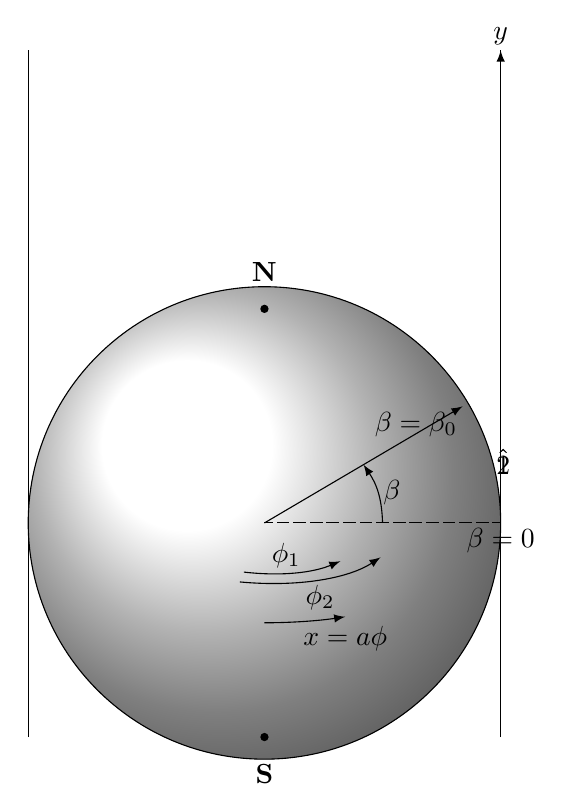
\begin{tikzpicture} % MERC

%% some definitions

\def\R{3} % sphere radius
\def\angEl{25} % elevation angle
\def\angAz{-100} % azimuth angle
\def\angPhiOne{-50} % longitude of point P
\def\angPhiTwo{-35} % longitude of point Q
\def\angBeta{33} % latitude of point P and Q

%% working planes

\pgfmathsetmacro\H{\R*cos(\angEl)} % distance to north pole
\LongitudePlane[xzplane]{\angEl}{\angAz}
\LongitudePlane[pzplane]{\angEl}{\angPhiOne}
\LongitudePlane[qzplane]{\angEl}{\angPhiTwo}
\LatitudePlane[equator]{\angEl}{0}

%% draw background sphere

\fill[ball color=white] (0,0) circle (\R); % 3D lighting effect
%\fill[white] (0,0) circle (\R); % just a white circle
\draw (0,0) circle (\R);

%% characteristic points

\coordinate (O) at (0,0);
\coordinate[mark coordinate] (N) at (0,\H);
\coordinate[mark coordinate] (S) at (0,-\H);
\path[xzplane] (\R,0) coordinate (XE);
\path[pzplane] (\angBeta:\R) coordinate (P);
\path[pzplane] (\R,0) coordinate (PE);
\path[qzplane] (\angBeta:\R) coordinate (Q);
\path[qzplane] (\R,0) coordinate (QE);

%% meridians and latitude circles

% \DrawLongitudeCircle[\R]{\angAz} % xzplane
% \DrawLongitudeCircle[\R]{\angAz+90} % yzplane
\DrawLongitudeCircle[\R]{\angPhiOne} % pzplane
\DrawLongitudeCircle[\R]{\angPhiTwo} % qzplane
\DrawLatitudeCircle[\R]{\angBeta}
\DrawLatitudeCircle[\R]{0} % equator

% shifted equator in node with nested call to tikz 
% (I didn't know it's possible)
\node at (0,1.6*\R) { \tikz{\DrawLatitudeCircle[\R]{0}} };

%% draw lines and put labels

\draw (-\R,-\H) -- (-\R,2*\R) (\R,-\H) -- (\R,2*\R);
\draw[->] (XE) -- +(0,2*\R) node[above] {$y$};
\node[above=8pt] at (N) {$\mathbf{N}$};
\node[below=8pt] at (S) {$\mathbf{S}$};
\draw[->] (O) -- (P);
\draw[dashed] (XE) -- (O) -- (PE);
\draw[dashed] (O) -- (QE);
\draw[pzplane,->,thin] (0:0.5*\R) to[bend right=15]
    node[midway,right] {$\beta$} (\angBeta:0.5*\R);
\path[pzplane] (0.5*\angBeta:\R) node[right] {$\hat{1}$};
\path[qzplane] (0.5*\angBeta:\R) node[right] {$\hat{2}$};
\draw[equator,->,thin] (\angAz:0.5*\R) to[bend right=30]
    node[pos=0.4,above] {$\phi_1$} (\angPhiOne:0.5*\R);
\draw[equator,->,thin] (\angAz:0.6*\R) to[bend right=35]
    node[midway,below] {$\phi_2$} (\angPhiTwo:0.6*\R);
\draw[equator,->] (-90:\R) arc (-90:-70:\R) node[below=0.3ex] {$x = a\phi$};
\path[xzplane] (0:\R) node[below] {$\beta=0$};
\path[xzplane] (\angBeta:\R) node[below left] {$\beta=\beta_0$};

\end{tikzpicture}


\begin{tikzpicture} % KART

\def\R{2.5}

\node[draw,minimum size=2cm*\R,inner sep=0,outer sep=0,circle] (C) at (0,0) {};
\coordinate (O) at (0,0);
\coordinate[mark coordinate] (Phat) at (20:2.5*\R);
\coordinate (T1) at (tangent cs: node=C, point={(Phat)}, solution=1);
\coordinate (T2) at (tangent cs: node=C, point={(Phat)}, solution=2);
\coordinate[mark coordinate] (P) at ($(T1)!0.5!(T2)$);

\draw[dashed] (T1) -- (O) -- (T2) -- (Phat) -- (T1) -- (T2);
\draw[<->] (0,1.5*\R) node[above] {$y$} |- (2.5*\R,0) node[right] {$x$};
\draw (O) node[below left] {$\mathbf{O}$} -- (P)
    +(1ex,0) node[above=1ex] {$\mathbf{P}$};
\draw (P) -- (Phat) node[above=1ex] {$\mathbf{\hat{P}}$};

\end{tikzpicture}
\end{comment}

\end{document} 
